\subsubsection{Детекция притока по данным температуры оптического кабеля}

\paragraph{Постановка задачи}
\par
Рассматривается вертикальная скважина L1. Для анализа доступны данные температуры, полученные с помощью волоконно-оптического кабеля, протянутого по длине скважины. Показания записывались в диапазоне порядка шести часов с шагом примерно 7 секунд – всего около 3000 измерений для участка траектории порядка 2.5км с шагом 0.5м. Пример данных в начале, в середине и в конце измерений показан на рис.\ref{fig:leakage_data}.

\begin{figure}[H]
\centering
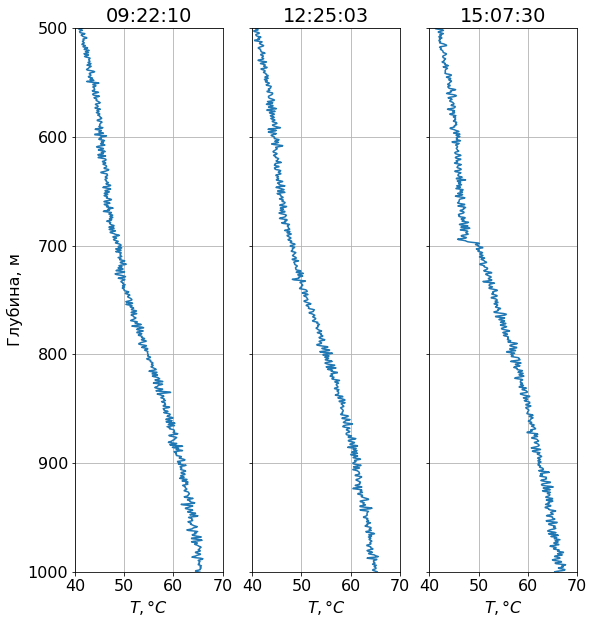
\includegraphics[width=0.8\textwidth]{PLT/leakage_data.png}
\caption{Пример данных в три различных периода времени. На третьем графике виден пик в районе 700м, на других двух он незаметен. Задача состоит в том, чтобы по всем сигналам выловить возможные пики, которые могут наблюдаться не на всем времени измерений.}
\label{fig:leakage_data}
\end{figure}

\par
Необходимо по всем доступным данным локализовать возможные места притока в скважине. Отклик от притока – температурная аномалия.

\paragraph{Методы и результаты}
\par
На предыдущем рисунке видно, что по последнему измерению можно заметить скачок температурных измерений на глубине порядка 700 м, в то время как на других двух ничего такого заметить нельзя. Данные шумные, однообразные и их много – поэтому для минимизации шума можно просто их усреднить – результат показан на рис.\ref{fig:leakage_results}(a).
\par
В полученном сигнале видно уже два скачка – на глубине порядка 700 и 1600, но они все еще слабые. Поэтому необходимо вычесть «гладкий» профиль сигнала и рассматривать только остаточный «шум». В качестве метода получения гладкого профиля выбрали кусочно-непрерывную аппроксимацию сплайнами третьей степени. После вычитания аппроксимации сплайнами остается сигнал, показанный на рис.\ref{fig:leakage_results}(b) – здесь скачки уже видны гораздо лучше.
\par
Тем не менее, в сигнале наблюдается низкочастотная осциллирующая структура, которая может быть артефактом измерений. Она автоматически убирается с помощью высокочастотного фильтра на основе преобразования Фурье (зануление в спектре всех частот ниже той, которая имеет максимальную интенсивность, и последующее восстановление сигнала). Спектр и остаточный сигнал показаны на рис.\ref{fig:leakage_results}(c),(d).
\par
Чтобы получить из данного сигнала некоторое подобие вероятности, позволяющее ранжировать только самые интересные участки, можно возвести модуль этого сигнала в какую-нибудь степень $\alpha, 1<\alpha<5$. Результат возведения в степень с $\alpha=4$ отнормирован на интервал [0,1] и показан на рис.\ref{fig:leakage_results}(e). Полученные пики для координат около 700 и 1600 локализуют места притока, а их амплитуды - «вероятность» – притока.

\begin{figure}[H]
\centering
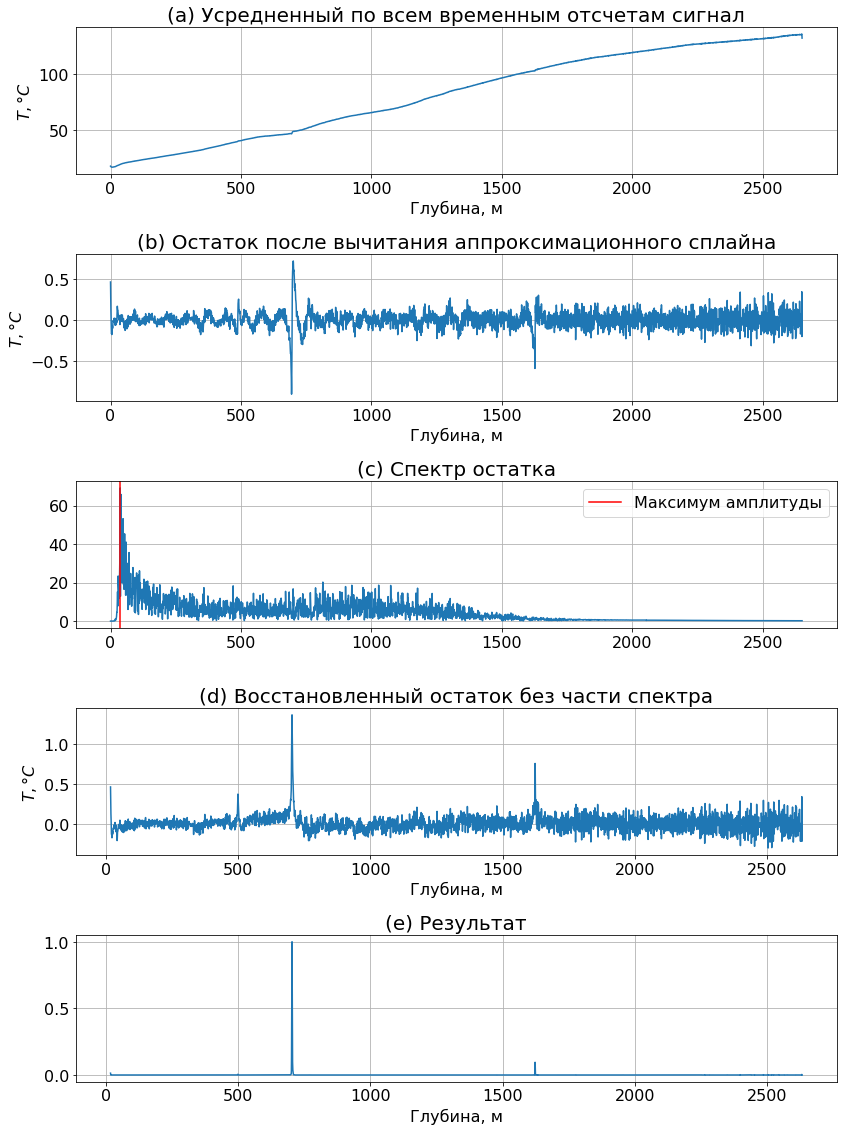
\includegraphics[width=1.0\textwidth]{PLT/leakage_results.png}
\caption{Последовательные этапы выделения полезной информации из усредненного сигнала.}
\label{fig:leakage_results}
\end{figure}